% This file was created with tikzplotlib v0.10.1.
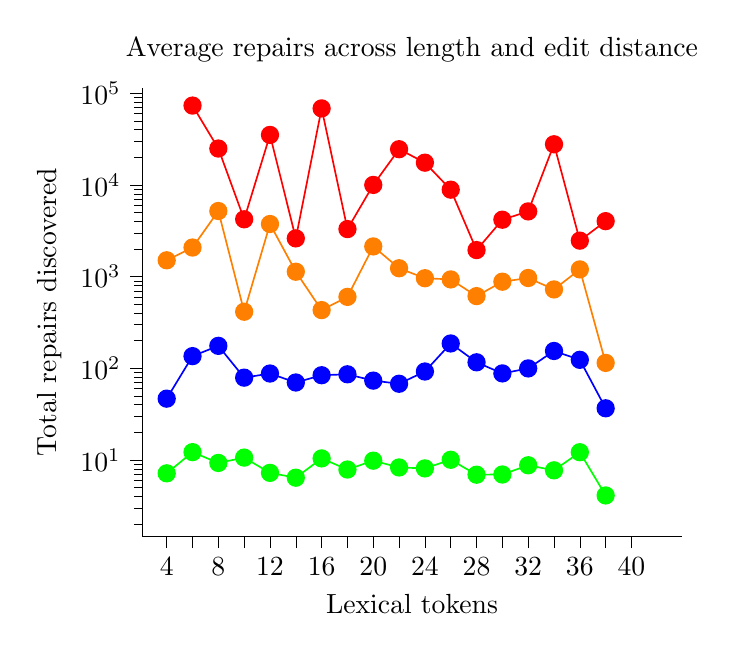
\begin{tikzpicture}
\begin{axis}[
  legend cell align={left},
  legend style={fill opacity=0.8, draw opacity=1, text opacity=1, draw=lightgray204},
  tick align=outside,
  tick pos=left,
  axis lines*=left,
  title={Average repairs across length and edit distance},
  x grid style={darkgray176},
  xlabel={Lexical tokens},
  xmin=-0.95, xmax=19.95,
  xtick style={color=black},
  xtick={0,1,2,3,4,5,6,7,8,9,10,11,12,13,14,15,16,17,18},
  xticklabels={4, , 8, , 12, , 16, , 20, , 24, , 28, , 32, , 36, , 40},
  y grid style={darkgray176},
  ylabel={Total repairs discovered},
  ymin=0, ymax=114560.263215582,
  ymode=log,
  legend pos=north east,
  ytick style={color=black}
]
\addplot [semithick, blue, mark=*, mark size=3, mark options={solid}]
table {%
0 46.625
1 135.653846153846
2 175.676923076923
3 79.0090909090909
4 87.6589147286822
5 69.9683544303797
6 83.9896373056995
7 85.9777777777778
8 73.3684210526316
9 67.7715517241379
10 92.1878172588832
11 186.568527918782
12 116.195945945946
13 87.8901734104046
14 99.6514285714286
15 154.44
16 123.658064516129
17 36.6111111111111
};
\addplot [semithick, orange, mark=*, mark size=3, mark options={solid}]
table {%
0 1506.8
1 2076.57142857143
2 5194.91304347826
3 413.939393939394
4 3749.34693877551
5 1130.83076923077
6 431.141025641026
7 601.172839506173
8 2135.26666666667
9 1233.85106382979
10 960.263888888889
11 932.225352112676
12 612.833333333333
13 880.2625
14 965.863636363636
15 725.139784946237
16 1199.05882352941
17 114.5
};
\addplot [semithick, green, mark=*, mark size=3, mark options={solid}]
table {%
0 7.14285714285714
1 12.1666666666667
2 9.27272727272727
3 10.6041666666667
4 7.22857142857143
5 6.4
6 10.3956043956044
7 7.86075949367089
8 9.81818181818182
9 8.28089887640449
10 8.08695652173913
11 10.0430107526882
12 6.90476190476191
13 6.94029850746269
14 8.74698795180723
15 7.70422535211268
16 12.1414141414141
17 4.1
};
\addplot [semithick, red, mark=*, mark size=3, mark options={solid}]
table {%
0 nan
1 73461
2 24965
3 4220.4
4 35145.8181818182
5 2613.28571428571
6 68402.25
7 3300.5
8 10010
9 24536.5217391304
10 17497.6315789474
11 8883.58333333333
12 1948.23076923077
13 4175.27272727273
14 5145.45454545455
15 27785.8095238095
16 2468
17 4027.25
};
\end{axis}

\end{tikzpicture}